\documentclass[conference]{IEEEtran}
\IEEEoverridecommandlockouts
\usepackage{cite}
\usepackage{balance}
\usepackage{amsmath,amssymb,amsfonts}
\usepackage{graphicx}
\usepackage{textcomp}
\usepackage{xcolor}
\usepackage{booktabs}
\usepackage{url}
\usepackage{array}
\usepackage{multirow}
\def\BibTeX{{\rm B\kern-.05em{\sc i\kern-.025em b}\kern-.08em\kern-.1667em\lower.7ex\hbox{E}\kern-.125emX}}
\begin{document}

\title{Context Sensitivity and Correlation Balancing for Motif-Driven Toxicity Prediction on Tox21}

\author{\IEEEauthorblockN{1\textsuperscript{st} Mehrdad Ghassabi}
\IEEEauthorblockA{\textit{Faculty of Computer Engineering}\\
\textit{University of Isfahan}\\
Isfahan, Iran\\
m.ghassabi@eng.ui.ac.ir}
\and
\IEEEauthorblockN{2\textsuperscript{nd} Sadra Hakim}
\IEEEauthorblockA{\textit{School of Computer Science}\\
\textit{University of Windsor}\\
Windsor, Canada\\
hakim6@uwindsor.ca}}

\maketitle

\begin{abstract}
Structural motifs can correlate with assay labels in molecular property prediction without fully explaining the endpoint, raising the possibility that models exploit such associations as shortcuts. We present an exploratory audit of this issue on the Tox21 benchmark. Using 2,048-bit Morgan fingerprints and five-fold structure-grouped cross-validation (Bemis--Murcko scaffolds, with Butina clustering for acyclic molecules), we compare Random Forest, Extra Trees, XGBoost, LightGBM, and a multilayer perceptron across all 12 assays and six SMARTS-defined motifs. Within-motif ROC-AUC was highest for Extra Trees (mean 0.680 over 41 eligible motif--assay groups) and Random Forest (0.674), and alkyl-halide-positive molecules were ranked best (0.739 and 0.737), whereas the MLP was weakest (0.592). We then defined a direction-based motif--label conflict subgroup and evaluated two interventions for alkyl-halide features on SR-ARE: approximate fingerprint-bit masking and correlation-balanced sample weighting. Bit masking produced at most a small conflict log-loss gain (RF, +0.024) and lowered overall ROC-AUC for all three tree models. Correlation balancing reduced conflict log loss by 0.54--0.61, but increased overall log loss by 0.11--0.18, a trade-off rather than evidence of improved generalization. We also show that the conflict rule can misassign expected labels under class imbalance, and we outline how to redesign it. These results underline the need for carefully defined subgroups when auditing shortcut behavior in toxicity prediction.
\end{abstract}

\begin{IEEEkeywords}
Molecular property prediction, toxicity prediction, shortcut learning, Tox21, Morgan fingerprints, correlation balancing, robustness, subgroup evaluation
\end{IEEEkeywords}

\section{Introduction}
Machine-learning systems can exploit predictive regularities that perform well under familiar conditions but fail when those regularities change. This behavior is often discussed as \emph{shortcut learning} \cite{geirhos2020}. In molecular-property prediction, the presence of a structural motif can correlate with a biological assay label without being a complete explanation of the endpoint. The association may vary with chemical environment, assay, and dataset composition. Therefore, a motif--label correlation or high predictive score is not itself evidence of a causal toxicological mechanism.

Tox21 contains multiple binary assay endpoints and is widely used in molecular machine-learning research \cite{richard2021,wu2018}. Morgan fingerprints encode atom-centered local environments \cite{rogers2010}, while tree ensembles and neural networks provide different learning procedures over the same representation. Aggregate performance can hide subgroup behavior, but subgroup analysis itself must be defined carefully: a rule that labels cases as agreement or conflict based only on the sign of an association can fail to capture the conditional label distribution.

This paper documents the progression from an initial within-motif discovery screen to a full 12-assay, five-model analysis. We treat the study as exploratory because the conflict-label rule has limitations and the experiments do not provide a causal test of internal model reliance. Our contributions are as follows.
\begin{enumerate}
\item A harmonized pipeline for all 12 Tox21 assays and five fingerprint models, with structure-grouped cross-validation that clusters acyclic molecules instead of collapsing them into a single group.
\item A within-motif context-sensitivity analysis over six SMARTS-defined motifs, which identifies alkyl halides as the most predictable motif.
\item An operational direction-based motif--label conflict analysis, together with an explicit account of where the rule fails.
\item A comparison of two interventions for alkyl-halide features, approximate fingerprint-bit masking and correlation-balanced training, including their effect on overall probability quality.
\end{enumerate}

\section{Related Work}
Shortcut learning describes predictive strategies that exploit signals that may not generalize robustly \cite{geirhos2020}. Molecular benchmarks such as MoleculeNet demonstrate that reported performance depends on the dataset, representation, and split strategy \cite{wu2018}. Extended-connectivity fingerprints encode molecular neighborhoods around atoms \cite{rogers2010}. Random Forest, Extra Trees, gradient boosting, and multilayer perceptrons are widely used learning approaches, but their algorithmic diversity alone does not guarantee robustness \cite{breiman2001,geurts2006,chen2016,ke2017}. Bemis--Murcko scaffolds summarize core frameworks; acyclic molecules often lack a non-empty scaffold, which requires an explicit grouping strategy \cite{bemis1996}.

\section{Study Design}
The study has two sequential components. First, a prior Random Forest screen evaluated within-motif discrimination across all 12 Tox21 assays and nominated alkyl halides for follow-up. Second, the full multi-model notebook applied a harmonized data-cleaning and cross-validation pipeline to all 12 assays with five fingerprint models. The first screen and the harmonized run have different duplicate-handling and evaluation details; their numbers are reported separately and should not be interpreted as a strict replication.

\section{Methods}
\subsection{Dataset and Label Harmonization}
The full-run notebook loaded 7,831 source rows from the Tox21 CSV, excluded eight invalid SMILES strings, canonicalized valid molecules using RDKit, and retained 7,823 unique valid structures. For each canonical structure and assay, a label was retained only if all non-missing duplicate labels agreed; conflicting labels were set to missing. The counts of observed labels were: NR-AR 7,258; NR-AR-LBD 6,751; NR-AhR 6,542; NR-Aromatase 5,815; NR-ER 6,186; NR-ER-LBD 6,948; NR-PPAR-gamma 6,443; SR-ARE 5,825; SR-ATAD5 7,065; SR-HSE 6,460; SR-MMP 5,804; and SR-p53 6,767. These correspond to 77,864 observed molecule--assay labels.

\subsection{Molecular Representation and Candidate Motifs}
All five models used 2,048-bit Morgan fingerprints with radius 2 \cite{rogers2010}. Six SMARTS patterns were tested: nitro, aldehyde, sulfonamide, aromatic amine, alkyl halide, and epoxide-like. These are operational definitions for subgroup analysis, not validated toxicophores. Alkyl halide was nominated from the discovery stage. The fingerprint-ablation method identified Morgan bit environments intersecting atoms in matched alkyl-halide substructures in the training fold. Because hashed bits can represent multiple environments, this is approximate ablation rather than a perfectly isolated chemical intervention.

\subsection{Structural Groups and Cross-Validation}
The full-run notebook used five-fold StratifiedGroupKFold with random state 20261017, varying the seed by assay. Non-empty Bemis--Murcko scaffolds were kept together. Of 7,823 structures, 1,775 had empty Bemis--Murcko scaffolds; these were assigned to Butina clusters of Morgan fingerprints at a Tanimoto similarity threshold of 0.60. The data contained 2,403 non-empty scaffold groups, 1,095 acyclic similarity clusters, and 3,498 structural groups in total. The selected clustering threshold has not yet been examined in a sensitivity analysis.

\subsection{Models}
The compared models were Random Forest (RF), Extra Trees, XGBoost, LightGBM, and a multilayer perceptron (MLP). RF and Extra Trees used 250 trees, minimum leaf size 2, and square-root feature subsampling. XGBoost used 250 estimators, depth 5, learning rate 0.05, row and feature subsampling of 0.8, and histogram tree construction. LightGBM used 250 estimators, learning rate 0.05, 31 leaves, and feature subsampling of 0.8. The MLP used hidden layers of 256 and 128 units, a training-fold-fitted standard scaler, early stopping, and a maximum of 100 iterations. These fixed settings were not selected by hyperparameter search. The optional graph model (Chemprop D-MPNN) was disabled and is not part of the reported results.

\subsection{Stage I: Within-Motif Context Sensitivity}
For every model, assay, and motif, ROC-AUC was computed among held-out molecules containing that motif. A motif--assay group was eligible if it contained at least 10 positive and 10 negative labels. This analysis asks whether the model can rank examples within a motif-positive subgroup; it does not by itself show shortcut reliance. The harmonized run returned 41 eligible motif--assay groups for each of the five models (205 model--group results total).

\subsection{Stage II: Direction-Based Motif--Label Conflict}
For each training fold and motif, the notebook calculated
\begin{equation}
\Delta=P(Y=1\mid M=1)-P(Y=1\mid M=0),
\end{equation}
where $M$ is motif presence and $Y$ is the binary assay label. The association was eligible when each motif-presence group had at least 25 training examples and $|\Delta|\geq0.10$. In the saved notebook, the expected binary label was set to $M$ when $\Delta>0$ and to $1-M$ otherwise; held-out labels were then used to partition eligible observations into agreement and conflict groups. Observations from folds failing association eligibility were excluded from these subgroup comparisons. A Laplace-smoothed motif-only baseline was calculated using training-fold label rates.

This operational rule is a key limitation. The sign of $\Delta$ indicates which motif group has the higher positive-label rate, but it does not establish that the higher-rate group has a positive majority or that the lower-rate group has a negative majority. The rule can therefore assign expected labels poorly under class imbalance. Moreover, conflict cases are by construction the labels that run against the training-fold trend, so elevated log loss in this group is partly expected. In the results, several motif--assay pairs show lower log loss in the nominal conflict group than in the agreement group, and some subgroup ROC-AUC values are undefined because only one class is represented. We report the notebook's outputs transparently but do not interpret the conflict partition as a validated measure of a shifted label relationship.

\subsection{Stage III: Mitigation and Uncertainty}
Mitigation was evaluated for RF, XGBoost, and LightGBM for the nominated alkyl-halide motif. The first method masked fingerprint bits whose training-fold atom environments overlapped alkyl-halide atoms. The second, correlation balancing, reweighted the four motif-presence-by-label cells; training weights were used only when every cell contained at least 10 examples, capped at 8, and normalized to mean 1. Positive conflict log-loss improvement is defined as full-model log loss minus intervention log loss. Overall ROC-AUC change is intervention minus full-model ROC-AUC. Overall log-loss change for balancing is intervention minus full-model log loss on the same paired SR-ARE observations, so positive values indicate worse probability quality. Confidence intervals were calculated from 2,000 bootstrap resamples of structural groups in the SR-ARE conflict subset. They estimate sampling variability across the chosen groups, not across datasets, endpoints, or training seeds.

\section{Results}
\subsection{Initial Random Forest Discovery Screen}
The initial analysis returned 41 eligible motif--assay groups across six candidate motifs. Its mean within-motif ROC-AUC was 0.663, with an approximate group-bootstrap 95\% interval of 0.627--0.698. Alkyl halides had the highest descriptive mean ROC-AUC at 0.718 across 12 assays and were nominated for follow-up. These figures are from the earlier screening protocol and are reported separately from the harmonized full run.

\begin{table}[t]
\centering
\caption{Initial Random Forest within-motif screen across 12 Tox21 assays.}
\label{tab:initial}
\small
\begin{tabular}{lrr}
\toprule
Motif & Eligible groups & Mean ROC-AUC \\
\midrule
Alkyl halide & 12 & 0.718 \\
Aromatic amine & 12 & 0.687 \\
Nitro & 9 & 0.634 \\
Epoxide-like & 2 & 0.610 \\
Sulfonamide & 4 & 0.578 \\
Aldehyde & 2 & 0.554 \\
\midrule
Total / mean & 41 & 0.663 \\
\bottomrule
\end{tabular}
\end{table}

\subsection{Full Multi-Model Context-Sensitivity Results}
Across all 12 assays, the full run generated 389,320 out-of-fold records (one record per observed molecule--assay label and model). Each model had 41 eligible motif--assay groups. Table~\ref{tab:contextfull} reports the unweighted mean across these groups and the alkyl-halide mean across all 12 assays. Extra Trees had the highest overall eligible-group mean (0.680). Within alkyl-halide-positive molecules, Extra Trees (0.739) and RF (0.737) were similar; MLP had the lowest mean (0.635). These are descriptive averages, not a ranking supported by paired hypothesis tests.

\begin{table}[t]
\centering
\caption{Full-run within-motif context sensitivity across five fingerprint models.}
\label{tab:contextfull}
\small
\begin{tabular}{lrr}
\toprule
Model & Mean AUC  & Alkyl-halide mean AUC  \\
 & over 41 groups &  (12 assays) \\
\midrule
Extra Trees & 0.680 & 0.739 \\
RF & 0.674 & 0.737 \\
LightGBM & 0.654 & 0.707 \\
XGBoost & 0.653 & 0.677 \\
MLP & 0.592 & 0.635 \\
\bottomrule
\end{tabular}
\end{table}

\subsection{Conflict Analysis Across Eligible Motif--Assay Pairs}
% TODO: the text says ten combinations passed the fold-level rule, but Table III lists seven rows
% (and the text below also mentions NR-AhR/aldehyde, NR-AhR/epoxide-like and SR-MMP/epoxide-like,
% which are not in the table). Reconcile with the notebook output before submission.
Ten motif--assay combinations passed the notebook's fold-level eligibility rule for at least one eligible fold. Table~\ref{tab:allconflict} summarizes agreement and conflict counts and the mean conflict-minus-agreement log-loss gap averaged across the five models. The results show why the subgroup definition requires refinement: nominal conflict log loss was lower than agreement log loss for NR-AhR/aldehyde, NR-AhR/epoxide-like, and SR-MMP/epoxide-like. In those cases, the expected-label heuristic is not behaving as an intuitive agreement/conflict split. ROC-AUC is not reported for a subgroup when it has too few observations from one class.

\begin{table*}[t]
\centering
\caption{Eligible motif--assay pairs under the notebook's direction-based conflict rule. Counts are shared across models; log-loss gap is the mean across models of conflict minus agreement log loss. Positive gaps mean the nominal conflict group has worse log loss.}
\label{tab:allconflict}
\footnotesize
\begin{tabular}{llrrrc}
\toprule
Assay & Motif & Agreement $n$ & Conflict $n$ & Mean log-loss gap & Mean conflict AUC \\
\midrule
NR-AhR & Aromatic amine & 5,585 & 957 & +0.988 & 0.609 \\
NR-AhR & Nitro & 1,040 & 264 & +0.634 & 0.671 \\
SR-ARE & Alkyl halide & 1,815 & 456 & +1.423 & 0.743 \\
SR-ARE & Epoxide-like & 1,862 & 408 & +1.584 & 0.388 \\
SR-ARE & Nitro & 4,772 & 1,053 & +1.419 & 0.517 \\
SR-MMP & Nitro & 4,809 & 995 & +1.195 & 0.466 \\
SR-p53 & Epoxide-like & 5,022 & 381 & +2.225 & 0.594 \\
\bottomrule
\end{tabular}
\end{table*}

\subsection{Alkyl-Halide/SR-ARE Model Comparison}
For the nominated alkyl-halide/SR-ARE pair, 1,815 eligible observations were labeled agreement and 456 conflict under the notebook's rule. Among these conflict cases, full-model log loss was higher than agreement log loss for all five models (Table~\ref{tab:conflict}). The conflict-to-agreement gap ranged from 1.037 for RF to 2.808 for MLP. Conflict ROC-AUC ranged from 0.628 for MLP to 0.827 for RF. The full model had lower conflict log loss than the motif-only baseline for four models; MLP was worse than the baseline. These results are descriptive, and their interpretation depends on the validity of the direction-based subgroup rule.

\begin{table*}[t]
\centering
\caption{Alkyl-halide/SR-ARE comparison across five models under the notebook's conflict rule. Lower log loss is better. Full-versus-motif-only improvement equals motif-only conflict log loss minus full-model conflict log loss.}
\label{tab:conflict}
\footnotesize
\resizebox{\textwidth}{!}{%
\begin{tabular}{lrrrrrr}
\toprule
Model & Agreement LL & Conflict LL & Gap & Conflict AUC & Motif-only conflict LL & Full vs. motif-only improvement \\
\midrule
RF & 0.168 & 1.205 & +1.037 & 0.827 & 1.517 & +0.312 \\
Extra Trees & 0.162 & 1.210 & +1.048 & 0.811 & 1.517 & +0.307 \\
XGBoost & 0.164 & 1.241 & +1.078 & 0.739 & 1.517 & +0.276 \\
LightGBM & 0.152 & 1.295 & +1.143 & 0.710 & 1.517 & +0.221 \\
MLP & 0.229 & 3.037 & +2.808 & 0.628 & 1.517 & $-$1.520 \\
\bottomrule
\end{tabular}}
\end{table*}

\subsection{Mitigation Results}
For the three mitigation models, only the alkyl-halide/SR-ARE pair had non-empty eligible conflict cases (456 observations across 310 structural groups). Bit masking had a small conflict log-loss improvement for RF (+0.024; bootstrap 95\% interval 0.001--0.044), but did not improve this metric convincingly for LightGBM or XGBoost. Overall ROC-AUC decreased after masking for all three models: by 0.021 for RF, 0.042 for LightGBM, and 0.023 for XGBoost. Overall log loss also worsened for all three.

Correlation-balanced training reduced conflict log loss in the same subset by 0.575 for RF, 0.539 for LightGBM, and 0.612 for XGBoost; all three group-bootstrap intervals were above zero. However, overall SR-ARE log loss on the same 5,825 paired observations increased by 0.143, 0.114, and 0.178, respectively. Thus, the intervention sharply improved the selected conflict metric while degrading overall probability quality. This is a trade-off, not evidence of improved generalization.

\begin{table*}[t]
\centering
\caption{Full-run mitigation results for alkyl halides on SR-ARE. Conflict improvement is full-model minus intervention log loss (positive is better). Overall AUC change is intervention minus full AUC; overall log-loss change is intervention minus full log loss (positive is worse). Intervals use structural-cluster bootstrap resampling.}
\label{tab:mitigation}
\footnotesize
\begin{tabular}{llrrrr}
\toprule
Model & Intervention & Conflict improvement & 95\% interval & Overall AUC change & Overall log-loss change \\
\midrule
RF & Bit masking & +0.024 & [0.001, 0.044] & $-$0.021 & +0.009 \\
LightGBM & Bit masking & $-$0.028 & [$-$0.076, 0.015] & $-$0.042 & +0.026 \\
XGBoost & Bit masking & $-$0.009 & [$-$0.042, 0.023] & $-$0.023 & +0.011 \\
\midrule
RF & Correlation balancing & +0.575 & [0.517, 0.632] & -- & +0.143 \\
LightGBM & Correlation balancing & +0.539 & [0.469, 0.607] & -- & +0.114 \\
XGBoost & Correlation balancing & +0.612 & [0.541, 0.681] & -- & +0.178 \\
\bottomrule
\end{tabular}
\end{table*}

Figure~\ref{fig:rf-early} preserves the exploratory Random-Forest-only plot from the preceding notebook. Its preprocessing and structural-grouping protocol differs from the full run, and it did not produce usable bootstrap intervals; it is included for study history only. Figure~\ref{fig:summary} visualizes the present full-run SR-ARE results.

\begin{figure*}[t]
\centering
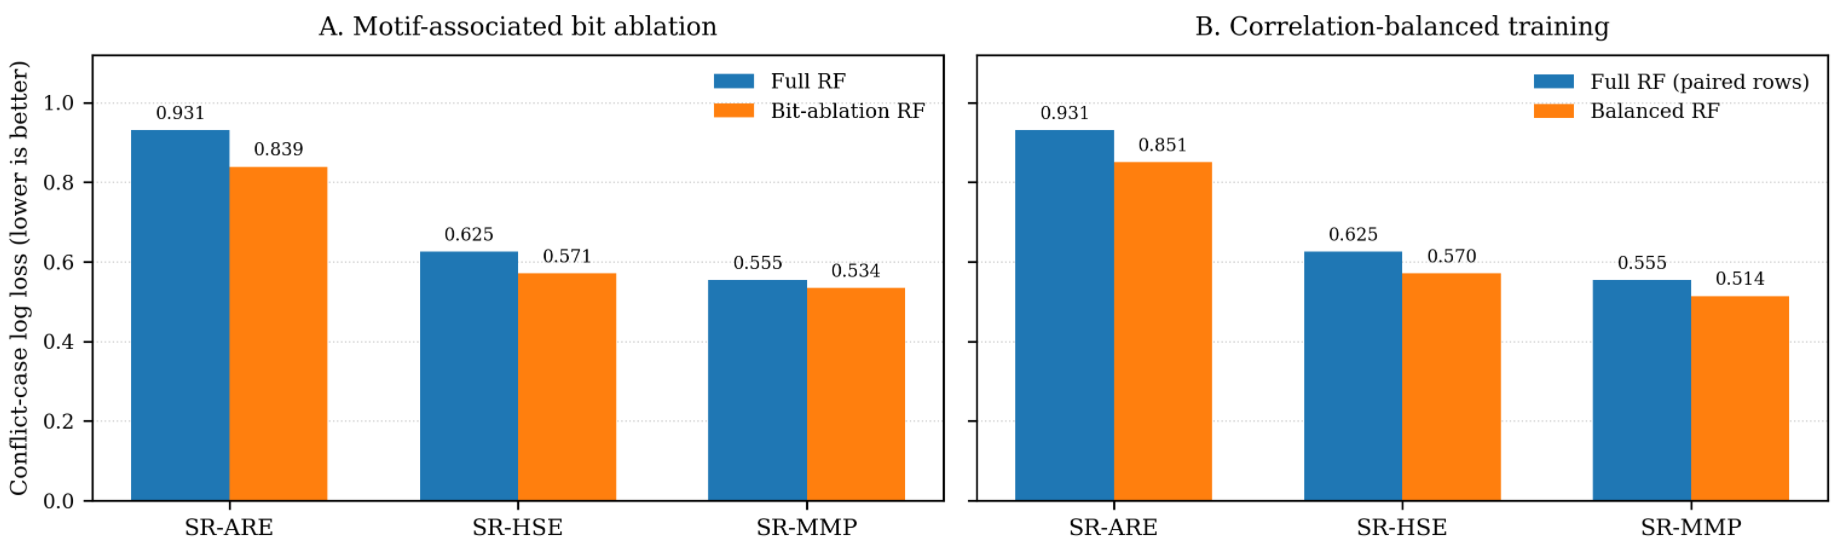
\includegraphics[width=0.98\textwidth]{fig1.png}
\caption{Historical Random-Forest-only visual summary from the earlier Notebook 2 analysis. Left: conflict-case log loss after motif-associated bit masking. Right: the full RF versus correlation-balanced training. These earlier values used a different analysis protocol and are not pooled with the full-run results in this paper.}
\label{fig:rf-early}
\end{figure*}

\begin{figure*}[t]
\centering
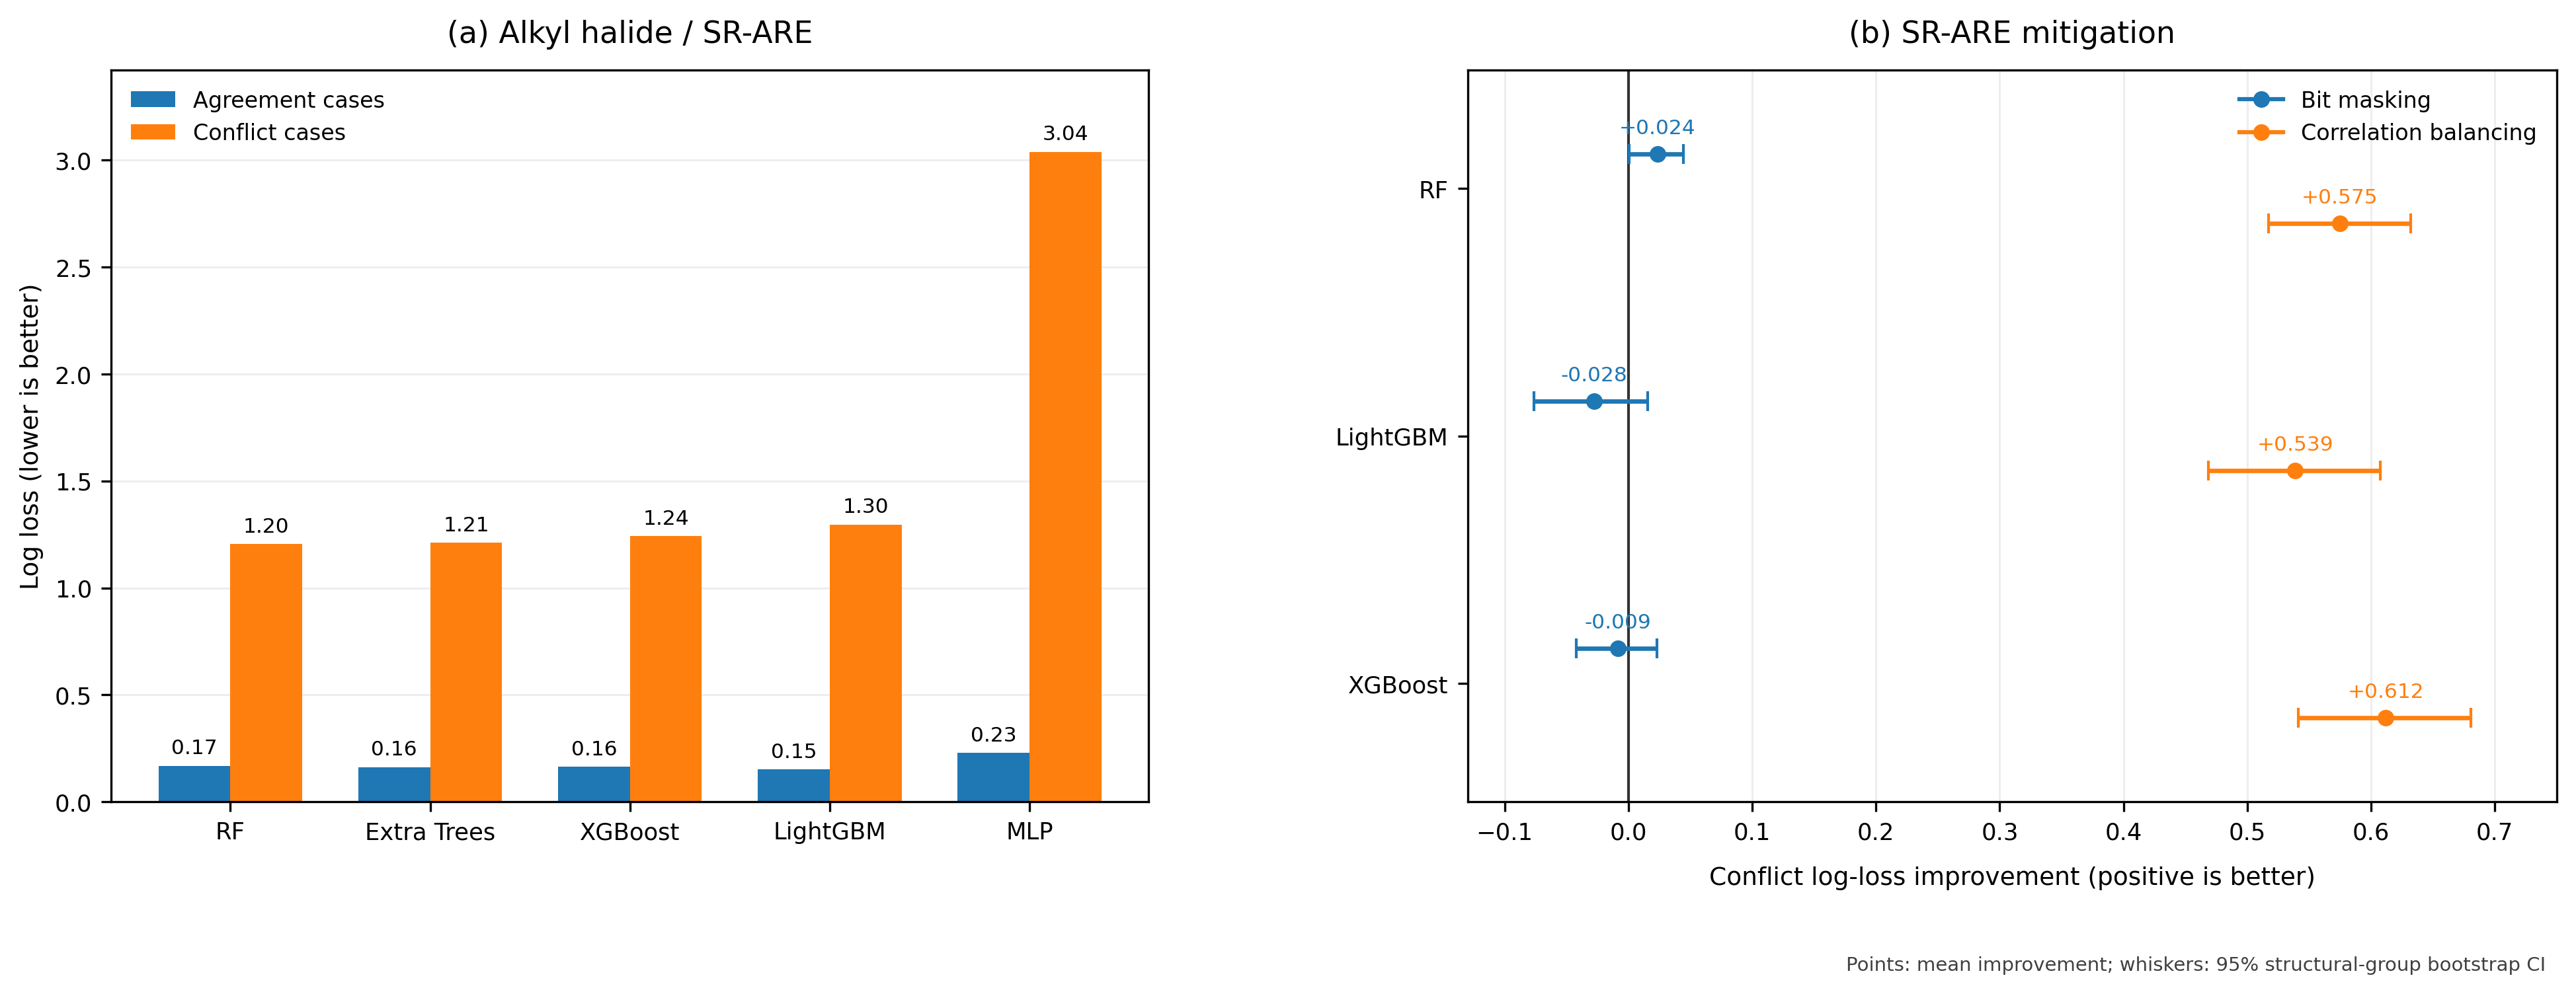
\includegraphics[width=0.98\textwidth]{fig2.png}
\caption{Visual summary using the completed five-fold, 12-assay full run. (a) Agreement and nominal conflict log loss for alkyl-halide/SR-ARE across five models under the notebook's direction-based rule. (b) Conflict log-loss improvement for RF, LightGBM, and XGBoost after bit masking and correlation balancing; error bars show structural-cluster bootstrap 95\% intervals. The large balancing improvements co-occur with worse overall log loss, and the subgroup rule's limitations are discussed in the text.}
\label{fig:summary}
\end{figure*}

\section{Discussion}
The full run extends the earlier Random Forest screen in two ways: it evaluates five learning algorithms across all 12 Tox21 assays, and it handles empty Bemis--Murcko scaffolds by clustering acyclic structures rather than collapsing all of them into one group. The context-sensitivity analysis found an average ROC-AUC of 0.680 for Extra Trees and 0.674 for RF across 41 eligible motif--assay groups. Alkyl halides had mean within-motif ROC-AUCs of 0.739 for Extra Trees and 0.737 for RF. These numbers suggest that predictive discrimination within the nominated motif is feasible, but they do not establish a shortcut.

The nominal alkyl-halide/SR-ARE conflict comparison shows a large log-loss gap across all five models, and the motif-only reference is outperformed by four of the five full models on that subgroup. However, the notebook's conflict rule is not yet sufficiently justified as an evaluation definition. It turns an association sign into an expected binary label without considering the actual conditional class rates. The negative agreement--conflict gaps for aldehyde and epoxide-like pairs and undefined subgroup AUCs are concrete warning signs. As a result, the current subgroup comparison should be treated as a debugging and hypothesis-generation result, not evidence that the models fail under a well-defined distribution shift.

Mitigation points to a metric trade-off. Bit masking yields a small positive conflict loss improvement for RF but worsens its overall AUC and log loss; it does not help LightGBM or XGBoost on conflict log loss. Correlation balancing reduces the selected conflict log loss substantially for all three models, but also raises overall log loss. Since the conflict cases were defined with a heuristic, even the large subgroup gains might partly reflect reweighting and calibration effects induced by the chosen partition. Balanced accuracy, precision, recall, F1, Brier score, calibration curves, and threshold-specific performance should be reported in future runs.

\section{Limitations and Next Steps}
First, the initial Random Forest screen and the harmonized five-model run differ in duplicate handling and evaluation configuration; the former is discovery evidence, not a strict replication. Second, the context-sensitivity statistic is calculated only for motif-positive groups containing at least 10 examples from each class. Third, the conflict heuristic needs redesign before its outcomes can be interpreted as a robust stress test. A better definition should use training-fold conditional probabilities explicitly and should not assume the majority class solely from the sign of $\Delta$; eligibility, binning, and outcome strata should be fixed before test analysis. Fourth, only SR-ARE yields an eligible alkyl-halide conflict subgroup for mitigation under the current rule. Fifth, bit masking can remove information from unrelated environments due to hashing. Sixth, the Butina threshold of 0.60 for acyclic grouping needs sensitivity analyses at alternative values. Seventh, models were not hyperparameter-tuned, only fingerprint representations were used, and no external dataset or independent endpoint was evaluated. The optional Chemprop graph model was not run.

Next steps are to correct and validate the conflict definition, preregister eligibility rules, test alternative acyclic clustering thresholds, add accuracy and calibration metrics, evaluate additional seeds, and then repeat the audit across all assays. A graph neural network and an external validation set should be included after the fingerprint-based protocol is stable. Until those checks are complete, conclusions should remain exploratory.

\section{Conclusion}
This study examined motif-associated behavior of fingerprint-based models on Tox21 under structure-grouped evaluation. Tree ensembles, particularly Extra Trees and Random Forest, discriminated best within motif-positive subgroups, and alkyl halides were the most predictable motif. A direction-based conflict analysis showed large log-loss gaps for the nominated alkyl-halide/SR-ARE pair. However, the subgroup definition proved unreliable in other motif--assay pairs, so we treat these gaps as hypothesis-generating rather than as evidence of failure under a well-defined distribution shift. Of the two interventions, bit masking offered little benefit and reduced overall performance, while correlation balancing sharply reduced conflict log loss at the cost of worse overall probability quality. Together, these findings suggest that improvements on a heuristically defined subgroup may reflect reweighting and calibration effects rather than reduced reliance on a shortcut. Future work should redefine conflict using training-fold conditional class rates, report calibration and threshold-based metrics, test sensitivity to the clustering threshold, add seeds and tuned baselines, and validate on external data and graph-based models before drawing mechanistic conclusions.

\section*{Data and Code Availability}
The full-run notebook used the public Tox21 CSV distributed via the DeepChem data endpoint. The notebooks and CSV outputs should be archived with versioned preprocessing, motif SMARTS, fold assignments, model settings, and all result tables in a persistent public repository before submission. A repository URL and data-access date should be added to the final manuscript; no public code repository is claimed in this draft.

\balance
\begin{thebibliography}{00}
\bibitem{geirhos2020}
R. Geirhos, J.-H. Jacobsen, C. Michaelis, R. Zemel, W. Brendel, M. Bethge, and F. A. Wichmann, ``Shortcut learning in deep neural networks,'' \textit{Nature Machine Intelligence}, vol. 2, pp. 665--673, 2020, doi: 10.1038/s42256-020-00257-z.

\bibitem{richard2021}
A. M. Richard \textit{et al.}, ``The Tox21 10K compound library: Collaborative chemistry advancing toxicology,'' \textit{Chemical Research in Toxicology}, vol. 34, no. 2, pp. 189--216, 2021, doi: 10.1021/acs.chemrestox.0c00264.

\bibitem{rogers2010}
D. Rogers and M. Hahn, ``Extended-connectivity fingerprints,'' \textit{Journal of Chemical Information and Modeling}, vol. 50, no. 5, pp. 742--754, 2010, doi: 10.1021/ci100050t.

\bibitem{breiman2001}
L. Breiman, ``Random forests,'' \textit{Machine Learning}, vol. 45, pp. 5--32, 2001, doi: 10.1023/A:1010933404324.

\bibitem{geurts2006}
P. Geurts, D. Ernst, and L. Wehenkel, ``Extremely randomized trees,'' \textit{Machine Learning}, vol. 63, pp. 3--42, 2006, doi: 10.1007/s10994-006-6226-1.

\bibitem{chen2016}
T. Chen and C. Guestrin, ``XGBoost: A scalable tree boosting system,'' in \textit{Proceedings of the 22nd ACM SIGKDD International Conference on Knowledge Discovery and Data Mining}, 2016, pp. 785--794, doi: 10.1145/2939672.2939785.

\bibitem{ke2017}
G. Ke, Q. Meng, T. Finley, T. Wang, W. Chen, W. Ma, Q. Ye, and T.-Y. Liu, ``LightGBM: A highly efficient gradient boosting decision tree,'' in \textit{Advances in Neural Information Processing Systems}, vol. 30, pp. 3146--3154, 2017.

\bibitem{bemis1996}
G. W. Bemis and M. A. Murcko, ``The properties of known drugs. 1. Molecular frameworks,'' \textit{Journal of Medicinal Chemistry}, vol. 39, no. 15, pp. 2887--2893, 1996, doi: 10.1021/jm9602928.

\bibitem{wu2018}
Z. Wu, B. Ramsundar, E. N. Feinberg, J. Gomes, C. Geniesse, A. S. Pappu, L. Leswing, and V. Pande, ``MoleculeNet: A benchmark for molecular machine learning,'' \textit{Chemical Science}, vol. 9, pp. 513--530, 2018, doi: 10.1039/C7SC02664A.
\end{thebibliography}
\end{document}